% Chapter 5

% variables
\newcommand{\pdirfive}{chapters/chapter5/plots}

\chapter{Future prospects} % Main chapter title
\label{chapter5} % For referencing the chapter elsewhere, use \ref{Chapter1} 

%----------------------------------------------------------------------------------------

\section{Micromegas upgrade}
\label{chapter5:sec:mm-upgrades}

\section{Calorimeter upgrade}
\label{chapter5:sec:cal-upgrades}

\section{Improvement to visible mode setup}
\label{chapter5:sec:new-vismode-setup}

\subsection{WCAL optimization}
\label{chapter5:sec:new-vismode-setup-wcal}

To design the new calorimeter structure, the figure of merit is the signal efficiency, which is defined mostly by the number of $\dm$ that decay outside the WCAL. This was quantified by a detailed MC-simulation of the setup used to generate the energy spectrum and the decay kinematics of the $\dm$.

%%% radiation length of tungsten collected at http://pdg.lbl.gov/2014/AtomicNuclearProperties/HTML/tungsten_W.html
In the design used in previous searches, the WCAL had 34 layers in total, each of them consisting of a converter layer made of 3 mm of tungsten and an active part made of a 2 mm plastic scintillators. This sums to a total of $\sim$30X$_0$. Reducing the dimension of the WCAL would impact the radiation length used to contain the main shower and hence change the background conditions. To avoid this, the new design of the calorimeter was studied under the principle that the optimal radiation length should be approximately 30X$_0$. The three following design were considered:

\begin{itemize}
\item An initial part of 9 layers using the original layer structure followed by an additional 25 layers of only tungsten.
\item A calorimeter consisting of 17 layers with layer-structure: 6mm tungsten + 2mm plastic scintillator.
\item A calorimeter consisting of 12 layers with a different structure: 9mm tungsten + 2mm plastic scintillator.
\end{itemize}

In all designs, the initial 5 layers forming the pre-shower part are still used for efficient hadron rejection. Despite its longer length, the first design grants a good energy resolution and a good hermeticity. In the second and third case, the calorimeter is more compact but has a worse energy resolution due to the thicker converter. A sketch of the two last designs is shown in Fig.\ref{fig:wcal-design} and compared to the original one used in the previous searches.

The third design was chosen to be the most suited for our search. The loss in energy resolution has almost no impact on the signal efficiency. The reason is that the short lifetime of the $\dm$ favors the detection of the ones produced at high energy that are able to escape the dump more efficiently. These $\dm$ carry most of the initial e$^-$ energy outside of the WCAL in the calorimeter placed downstream (ECAL). Hence, the energy is reconstructed with a precision of $<$1\% regardless of the WCAL structure. The second and third designs are compared to the original WCAL in Table \ref{tab:wcal-length-results}.

\iffalse
\begin{center}
\begin{table}[tbh!]
\begin{tabular}{lccr}
  WCAL structure [mm](layers) & WCAL length [mm] & $\epsilon$  & EOT to cover $\dm$ at 90\% confidence [$10^{10}$] \\
  \hline
  ECAL1:3+2(34)                & 178               & 0.001   & 17$\pm$3.4     \\ 
  ECAL1:6+2(17)                & 148               & 0.001   & 7$\pm$0.9      \\
  ECAL1:9+2(12)                & 138               & 0.001   & 6$\pm$0.7      \\
  ECAL1:3+2(34)                & 178               & 0.0012  & 85$\pm$4.7     \\
  ECAL1:6+2(17)                & 148               & 0.0012  & 24$\pm$6.9     \\  
  ECAL1:9+2(12)                & 138               & 0.0012  & 19$\pm$5       \\  
  \hline
\end{tabular}
\label{tab:wcal-length-results}
\caption{Number EOT required to cover $\dm$ at 90\% confidence using different WCAL designs in the visible mode setup proposed for 2021. The first entry describes the structure using the convention:
  ECALconverter-depth+counter-depth(number-of-layers).}
\end{table}
\end{center}
\fi

\begin{figure}[tbh!]
  \centering
  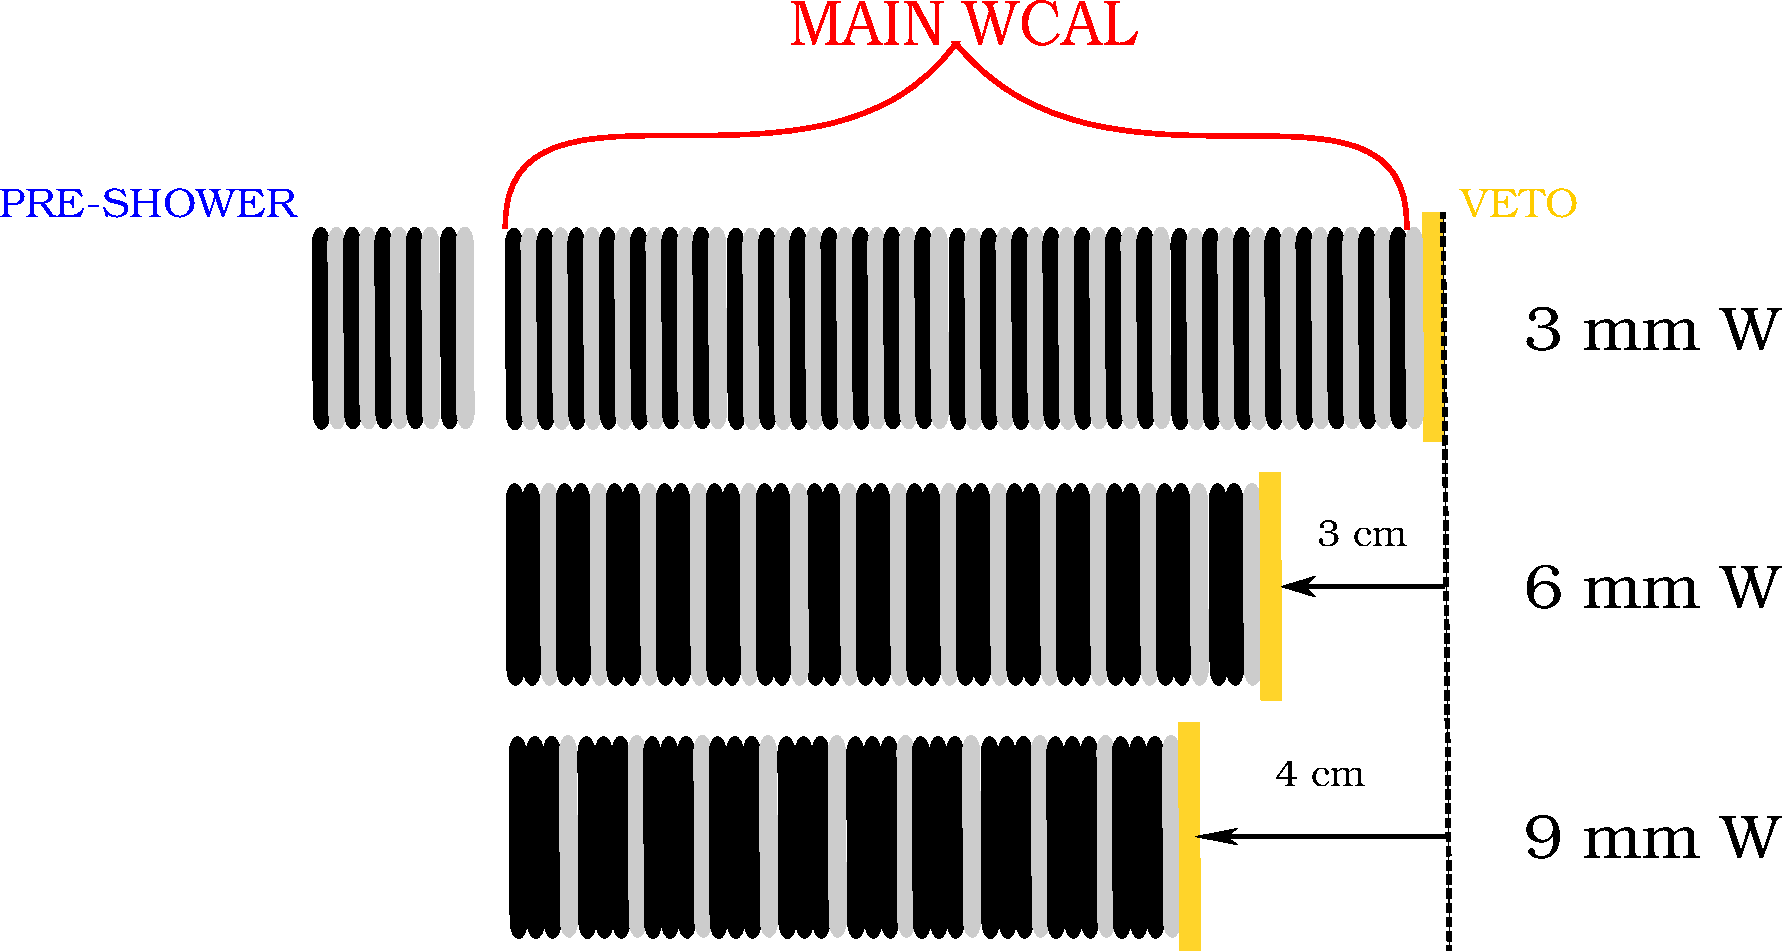
\includegraphics[scale=0.5]{\pdirfive/WCAL_design.pdf}
  \caption{Possible designs of the WCAL re-arranging the available tiles of 3 mm of Tungsten (W) and 2 mm of scintillator material. All designs posses the same radiation length of 30$X_0$.}
  \label{fig:wcal-design}
\end{figure}

\subsection{Invariant mass reconstruction}
\label{chapter5:sec:new-vismode-setup-invmass}

\section{A new approach: Muon mode setup}
\label{chapter5:sec:muon-mode-setup}
